	\chapter{Programmbeschreibung}\label{cha:program_description}
	In diesem Abschnitt soll eine Implementierung einiger der in den bisherigen Abschnitten vorgestellten Ideen in Form des Computerprogramms \texttt{PIRaTE} (=\texttt{P}ath \texttt{I}ntegral \texttt{Ra}diative \texttt{T}ransfer with \texttt{E}ase) vorgestellt werden. Dabei soll zum einen ein Überblick über das Programm durch eine abstrakte Modulbeschreibung gegeben werden. Zum anderen sollen aber auch atypische Implementierungsdetails herausgegriffen und vorgestellt werden.
	
	%TODO: Programmbeschreibung in Worten bzw. Pseudocode, Modulbeschreibung, Details in evtl. Anhang auslagern, Erhöhte Modularität beim robusten MH-Algo durch feste Mutationen, die über die Sample--Generierungsmethode adaptiv angepasst werden.
	
	\section{Allgemeines}
	\subsection{Programmiersprache}
	\pirate ist in der rein funktionalen Programmiersprache {\em Haskell} geschrieben. Funktionale Programmiersprachen bauen auf der Idee auf, Programme als Aneinanderreihung vieler kleiner Funktionen darzustellen, von denen jede Funktion eine bestimmte Aufgabe erfüllt. Das Ergebnis einer Funktion hängt dabei nur von den Eingabeparametern ab, d.h. gleiche Eingabewerte führen immer zum gleichen Rückgabewert, was genau der mathematischen Idee einer Funktion entspricht. Funktionen sind somit nebeneffektfrei, d.h. sie können weder auf Zustände (wie z.B. die Uhrzeit oder den Inhalt einer Datei) außerhalb ihrer Eingabeparameter zurückgreifen, noch können sie, vom Rückgabewert abgesehen, Einfluss auf den ``Zustand der Welt'' (d.h. den Inhalt von Dateien oder eine Ausgabe auf dem Bildschirm) nehmen.
	
	Die Hauptroutine stellt die übergeordnete Funktion dar, die Benutzereingaben oder Kommandozeilenargumente als Funktionsparameter bekommt und deren Rückgabewert die Programmausgabe ist.
	
	In Haskell existieren außerdem keine Variablen, sondern nur lokale Konstanten, d.h. Programme der Art
		\begin{algorithmic}
			\STATE $x\leftarrow 41$
			\STATE $x\leftarrow x+1$
		\end{algorithmic}
	sind in Haskell nicht zulässig, da keine Art von Zustandsspeicherung außer der Weitergabe als Funktionsparameter gestattet ist. Stattdessen wäre
		\begin{algorithmic}
			\STATE $x\leftarrow 41$
			\STATE $y\leftarrow x+1$
		\end{algorithmic}
	eine gültige Alternative. Was sich zunächst wie ein Nachteil anhört, vermeidet automatisch eine Vielzahl häufig auftretender Programmierfehler, deren Ursache darin liegt, dass die Möglichkeit, einer Variablen einen neuen Wert zuzuweisen, zwangsläufig mit sich bringt, dass die Ausführungsreihenfolge der Instruktionen die Bedeutung des Programms ändern kann. In Haskell wird hingegen die Ausführungsreihenfolge nicht durch den Programmierer spezifiziert, sondern lediglich die Abhängigkeiten der verschiedenen Berechnungen voneinander. Der Compiler kann die Aus\-führ\-ungs\-rei\-hen\-fol\-ge dann durch Auflösen der Abhängigkeiten selbst bestimmen.
	
	Eine weitere Besonderheit von Haskell besteht darin, dass standardmäßig Funktionen nur nach Bedarf ausgewertet werden, d.h. nicht dann wenn sie aufgerufen werden, sondern erst dann wenn der Wert später im Verlauf der Rechnung gebraucht wird. Dies erlaubt u.a. das Arbeiten mit unendlich großen Datenstrukturen (wie unendlich langen Listen) und eine einfachere Trennung des  Programmcodes in Teile zum ausschließlichen Generieren bzw. Konsumieren von Daten.
		
	Eine genauere Beschreibung von Haskell würde den Rahmen dieser Arbeit sprengen, deshalb sei für mehr Details auf die Webseite
	
	\url{http://www.haskell.org}
	
	verwiesen. Ein lesenswerter Essay von John Hughes zu den Vorteilen funktionaler Programmiersprachen ist:
	
	{\em Why Functional Programming Matters}
	
	\url{http://www.md.chalmers.se/~rjmh/Papers/whyfp.html}.
	
	
	\subsection{Funktionsumfang}
	\pirate ist in der Lage die relative Intensitätsverteilung über Pixel zu simulieren, die ein virtueller monochromatischer CCD--Sensor messen würde. Dazu nutzt es die in Abschnitt \ref{sec:robustmetropolis} vorgestellte Abwandlung des Metropolis--Hastings--Algorithmus, um mit einer Häufigkeit proportional zum Messbeitrag Photonenpfade zu ziehen.
	
	Für zukünftige Versionen ist geplant, den absoluten Fluss durch Monte--Carlo--Integration zu schätzen und zur Normierung der relativen Intensitätsverteilung über die Pixel zu nutzen. Außerdem soll \pirate auch polychromatische Probleme und Spektren berechnen können. Dies sollte mit relativ geringem Aufwand möglich sein. Interessant wäre darüber hinaus die von \citet{Liu:2000p8427} vorgeschlagene Erweiterung des Metropolis--Algorithmus zu implementieren, bei der mehrere Vorschlagssamples gezogen werden.
	
	\section{Modulbeschreibung}
	
	\pirate ist in verschiedene Module unterteilt. Die wichtigsten Module und ihre Ab\-hän\-gig\-kei\-ten sind in Abb.~\ref{fig:moduleoverview} dargestellt.
		\begin{figure}
				\centering
				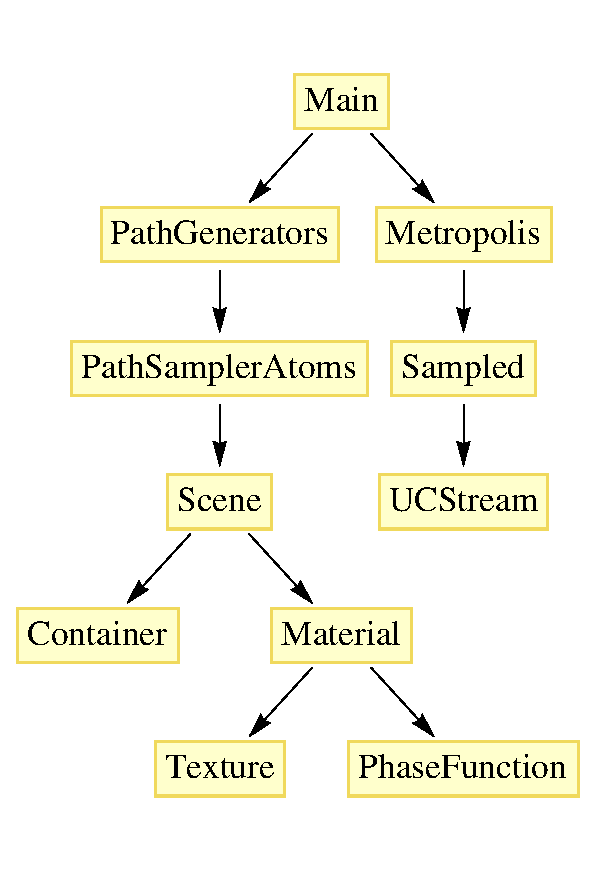
\includegraphics[height=0.3\textheight]{moduleoverview.eps}
				\caption{Illustration der Modulhierarchie in \texttt{PIRaTE}.}
				\label{fig:moduleoverview}
		\end{figure}
		%\begin{wrapfigure}{r}{0.6\textwidth}
		%	\centering
		%	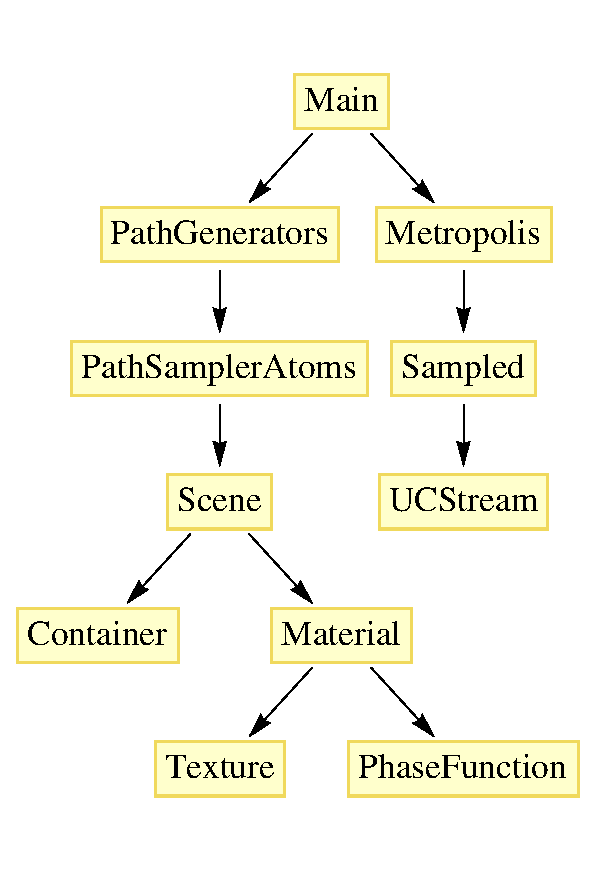
\includegraphics[height=0.2\textheight]{moduleoverview.eps}
		%	\caption{Modulhierarchie in \texttt{PIRaTE}.}
		%	\label{fig:moduleoverview}
		%\end{wrapfigure}
	Das Modul \textbf{Scene} erlaubt die Beschreibung eines konkreten Strahlungstransportproblems (im Folgenden Szene genannt) und stellt eine Schnittstelle zur Abfrage von Informationen innerhalb der Szene bereit. Eine Szene besteht dabei aus einer Liste von Containern, die mit einem oder mehreren Materialien gefüllt sein können. Ein Container repräsentiert ein (meist abgeschlossenes) Raumgebiet, z.B. eine Kugel oder ein Quader. Für jeden Container müssen dabei Funktionen implementiert sein, die angeben, ob ein Raumpunkt innerhalb des Containers liegt, ob und wo ein Strahl den Container schneidet, sowie eine Abbildung aus dem dreidimensionalen Einheitswürfel auf Raumpunkte innerhalb des Containers. Ein Material besteht aus Skalarfeldern für Absorptionquerschnitt, Streuquerschnitt, Emissivität und Sensitivität sowie getrennten Phasenfunktionen für Emission, Streuung und Sensation. Skalarfelder sind im Modul \textbf{Texture} definiert und erlauben sowohl homogene Skalarfelder mit einem konstanten Wert als auch inhomogene Skalarfelder, die durch eine beliebige Funktion aus $\mathbb{R}^3\to\mathbb{R}$ jedem Raumpunkt einen Wert zuordnen. Phasenfunktionen sind im Modul \textbf{Phasefunction} definiert. Wie bei Containern muss zur Definition einer Phasenfunktion eine Abbildung aus $[0,1]^2\to\mathcal{S}^2$ angegeben werden, die zwei Zahlen aus dem Einheitsintervall auf eine Raumrichtung abbilden. Nach der Definition einer Szene durch Kombination von Materialien und Containern stellt \textbf{Scene} eine Schnittstelle bereit, mit der sich punktuelle Eigenschaften, wie der Absorptionsquerschnitt, die Albedo, Emissivität oder eine Liste aller Streuphasenfunktionen an einem Ort abfragen lassen. Außerdem lassen sich optische Tiefen abfragen, entweder zwischen zwei Punkten oder von einem Punkt aus in eine bestimmte Raumrichtung, bis ein festgelegtes Distanz- oder optisches Tiefenziel erreicht ist. Zur Berechnung der optischen Tiefen wird entlang des Strahls eine Liste disjunkter Intervalle gefüllt mit homogenem Material berechnet. Ist eines der beteiligten Materialien inhomogen, wird es stückweise durch homogene Intervalle ersetzt, deren Werte durch Mittelung der inhomogenen Funktion mittels eines Gauss--Legendre--Verfahrens bestimmt werden.
	
	Auf diese Schnittstelle baut das Modul \textbf{PathSamplerAtoms} auf. Es stellt Methoden zum Samplen von Punkten, Richtungen und Distanzen für Emission, Streuung und Sensation bereit (s. Tab.~\ref{tab:pathsampleratoms}).
	\begin{table}[htdp]
		\caption{Alle neun vom Modul \textbf{PathSamplerAtoms} bereitgestellten Methoden. Der Pfeil beschreibt aus welchen Eingangswerten welches Ergebnis gezogen wird.}
		\begin{center}
		\begin{tabular}{|c|c|c|}
			\hline
			Punkt--Sampler & Richtungs--Sampler & Distanz--Sampler \\
			\hline
			Szene & (Szene,einfallender Strahl) & (Szene,ausgehender Strahl) \\
			$\downarrow$ & $\downarrow$ & $\downarrow$ \\
			Punkt & ausgehende Richtung & Distanz \\
			\hline\hline
			SensationPointSampler & SensationDirectionSampler & SensorDistanceSampler \\
			ScatteringPointSampler & ScatteringDirectionSampler & ScattererDistanceSampler \\
			EmissionPointSampler & EmissionDirectionSampler & EmitterDistanceSampler \\
			\hline
		\end{tabular}
		\end{center}
		\label{tab:pathsampleratoms}
	\end{table}%
	So erlaubt der {\em SensationPointSampler} aus einer Szene einen zufälligen Raumpunkt zu ziehen, der innerhalb eines der Container liegt, die ein sensitives Material beinhalten. Der {\em ScatteringDistanceSampler} erlaubt, aus einer Szene und einem einfallenden Strahl (d.h. einem Streuort und einer Richtung aus der das Photon kommt) eine ausgehende Richtung zu samplen, in die das Photon gestreut wird. Mithilfe des {\em EmitterDistanceSampler} lässt sich aus einer Szene, einem Ort und einer ausgehenden Richtung eine zufällige Distanz bis zum nächsten Emissionspunkt ziehen. Dabei werden beim Ziehen aus einem Punkt--Sampler die von den Containern bereitgestellten, obengenannten Abbildungen auf Punkte in ihrem Volumen benutzt. Ebenso greifen die Richtungs--Sampler auf die von den Phasenfunktionen am spezifizierten Ort bereitgestellten Abbildungen auf eine Richtung zurück. Der {\em ScatteringDirectionSampler} berücksichtigt außerdem die angegebene einfallende Richtung, {\em EmissionDirectionSampler} sowie {\em SensationDirectionSampler} können diese ignorieren, da Emission und Sensation terminale Prozesse sind, so dass nur eine Richtung in die jeweilige Phasenfunktion eingeht. {\em EmitterDistanceSampler} und {\em SensorDistanceSampler} implementieren den in Abschnitt \ref{subsubsec:distancesampler}  vorgestellten Distanzsampler $P_1$, {\em ScattererDistanceSampler} implementiert den Distanzsampler $P_3$. In der aktuellen Version von \pirate wird nicht von all diesen Samplern Gebrauch gemacht. Die Implementierung all dieser Sampler, erlaubt aber eine hohe Flexibilität und eine leichte Implementierung zukünftiger Pfadgenerierungsverfahren.
	
	Mithilfe der in \textbf{PathSamplerAtoms} bereitgestellten Grundbausteine wird im Modul \textbf{PathGenerators} das Verfahren zum Generieren kompletter Pfade aus Abschnitt \ref{subsec:sensor_based_raycasting} implementiert. Die Wahrscheinlichkeit $p_\text{grow}$, einen zu\-sätz\-lich\-en Streupunkt zu generieren, ist dabei ein freier Parameter, der für jede Simulation neu angegeben werden kann.
	
	Im Modul \textbf{Sampled} wird eine Schnittstelle für samplebare Objekte jeder Art definiert. Dies beinhaltet eine Funktion, die aus einem Strom aus Zufallszahlen ein Sample generieren kann, sowie Funktionen, um die entsprechende Wahrscheinlichkeitsdichte, sowie einen eventuellen Beitrag des Samples zu berechnen. Dies wird im Programm an allen Stellen benutzt, an denen zufällige Stichproben generiert werden, z.B. beim Samplen eines Punktes aus einem Container, dem Samplen einer Raumrichtung aus einer Phasenfunktion oder dem Samplen eines kompletten Pfades aus einer Pfadgenerierungsmethode. Im Fall eines Pfades ${\overline x}$, wird so neben dem Pfad als Sample auch das Verhältnis aus Messbeitragsfunktion $f({\overline x})$ und Generierungswahrscheinlichkeit $p({\overline x})$ berechnet. Durch die Möglichkeit, direkt das Verhältnis beider Ausdrücke zu berechnen, wird die Pfadgenerierung wesentlich effizienter, da sich viele gemeinsame Faktoren herauskürzen. Durch diese feste Schnittstelle ist es möglich, die Kombination einfacher Samplingmethoden zu komplexeren wieder auf eine Funktion zu reduzieren, die aus einer unendlich langen Liste von Zufallszahlen Samples generieren kann.
	
	Das \textbf{Metropolis}--Modul implementiert den in Abschnitt \ref{sec:robustmetropolis} vorgestellten abgewandelten Metropolis--Hastings--Algorithmus. Im Gegensatz zum klassischen MH--Algorithmus gewichten wir generierte Pfade aber nicht voll oder gar nicht (bei Ablehnung des Samples), sondern gewichten jedes Sample mit seiner Akzeptanzwahrscheinlichkeit. Dieses Vorgehen hat denselben Erwartungswert, nutzt aber auch die abgelehnten Samples, was zu einem effizienteren Verfahren führt. Hierdurch können insbesondere Pfade zur Konvergenz der Messung beitragen, die nur eine sehr geringe Wahrscheinlichkeit haben, gesampelt zu werden. In Pseudocode dargestellt sieht dies folgendermaßen aus:
	
	\begin{algorithmic}
		\REPEAT[finde beitragenden Pfad]
		\STATE $u \leftarrow$ Anfangszustand
		\STATE $x \leftarrow S(u)$
		\UNTIL{$f(x_1)>0$}
		\STATE $w = 1$ \COMMENT{Gewicht des aktuellen Samples}
		\FOR{$i=1$ to $N$}
			\STATE $r\leftarrow$ Zufallszahl aus $[0,1]$
			\IF[Mutation schlägt frisches Sample vor]{$r < p_\text{fresh}$}
				\STATE $T \leftarrow T_\text{fresh}$
			\ELSE[Mutation schlägt leicht abgewandeltes Sample vor]
				\STATE $T \leftarrow T_\text{perturb}$
			\ENDIF
			\STATE $u'\leftarrow$ ziehe Wert gemäß $T(u'|u)$
			\STATE $x' \leftarrow S(u')$
			\STATE $a(u'|u) \leftarrow \text{min}\left(1,\frac{f(x')}{f(x_i)}\right)$
			\STATE $r\leftarrow$ Zufallszahl aus $[0,1]$
			\IF{$r < a(u'|u)$}
				\STATE $x_i \leftarrow x$
			  \STATE $w_i \leftarrow w+(1-a(u'|u))$
				\STATE $u \leftarrow u'$
			  \STATE $x \leftarrow x'$
			  \STATE $w \leftarrow a(u'|u)$
			\ELSE
				\STATE $x_i \leftarrow x'$
				\STATE $w_i \leftarrow a(u'|u)$
				\STATE $w \leftarrow (1-a(u'|u))$
			\ENDIF
	  \ENDFOR
	  \STATE\COMMENT{gebe Liste gewichteter Samples zurück}
	  \RETURN{$(w,x)$}
	\end{algorithmic}
	
	Im Modul \textbf{UCStream} (={\em UnitCoordinatesStream}) werden Funktionen zum Generieren dieser unendlich langen Listen aus Zufallszahlen definiert. Darüber hinaus werden auch Funktionen zur Variation eines solchen Zufallszahlenstroms durch kleine zufällige Störungen mit einem anderen Zufallszahlenstrom definiert.
	
	Das Modul \textbf{Main} ruft den Metropolis--Algorithmus mit dem Pfadgenerierungsverfahren aus \textbf{PathGenerators} auf und extrahiert aus der Liste gewichteter Pfade die Verteilung der Pfade über den virtellen CCD--Sensor und gibt das durch Binning entstehende Bild in eine Datei aus.
	
	Der Quellcode von \pirate ist unter
	
	\url{http://github.com/theidecke/PIRaTE}
	
	öffentlich zugänglich.
	
	
	
	
	